% Revised edition: 13 motivation frames inserted before the relevant concepts.
% See insertion_guide.md for original/revised page mapping and teaching prompts.
% COMP 5212 lecture deck: Rademacher Complexity and VC Dimension
% Core organization, definitions, theorems, and proof strategy follow Chapter 3 of:
% M. Mohri, A. Rostamizadeh, and A. Talwalkar,
% Foundations of Machine Learning, 2nd ed., MIT Press, 2018.
% Official author lecture slides were also consulted.
%
% Instructor-added material: pacing, checkpoint questions, geometric redraws,
% toy computations, and numerical examples.
%
% No external images are required. All diagrams are drawn in TikZ.
% The source uses explicit font sizes rather than oversized text commands.

\documentclass[aspectratio=169,10pt]{beamer}

\usepackage[T1]{fontenc}
\usepackage[utf8]{inputenc}
\usepackage{lmodern}
\usepackage{amsmath,amssymb,mathtools}
\usepackage{array,booktabs,multirow}
\usepackage{tikz}
\usetikzlibrary{arrows.meta,positioning,shapes.geometric,calc,fit,backgrounds,decorations.pathreplacing}
\usepackage{hyperref}

% -----------------------------------------------------------------------------
% Visual style: consistent with the earlier COMP 5212 decks
% -----------------------------------------------------------------------------
\definecolor{slideorange}{HTML}{D62B09}
\definecolor{bulletgreen}{HTML}{A8C9A0}
\definecolor{bulletgray}{HTML}{D9E1E8}
\definecolor{deepblue}{HTML}{234A84}
\definecolor{softblue}{HTML}{EAF1FA}
\definecolor{softorange}{HTML}{FBEDE7}
\definecolor{softgreen}{HTML}{EDF5EB}
\definecolor{softgray}{HTML}{F2F3F5}
\definecolor{midgray}{HTML}{666666}
\definecolor{darkgreen}{HTML}{2F7A45}
\definecolor{darkred}{HTML}{A1261A}
\definecolor{pointblue}{HTML}{4E79A7}
\definecolor{pointred}{HTML}{D95F59}
\definecolor{pointgold}{HTML}{D6A84B}

\hypersetup{colorlinks=true,urlcolor=deepblue,linkcolor=deepblue}
\urlstyle{same}

\setbeamertemplate{navigation symbols}{}
\setbeamercolor{background canvas}{bg=white}
\setbeamercolor{normal text}{fg=black,bg=white}
\setbeamercolor{frametitle}{fg=slideorange,bg=white}
\setbeamercolor{page number in head/foot}{fg=black,bg=white}
\setbeamercolor{block body}{bg=softblue,fg=black}
\setbeamercolor{block title}{bg=deepblue,fg=white}
\setbeamercolor{alerted text}{fg=darkred}
\setbeamerfont{frametitle}{series=\bfseries,size*={25pt}{29pt}}
\setbeamerfont{page number in head/foot}{size=\scriptsize}
\setbeamersize{text margin left=0.90cm,text margin right=0.90cm}

\setbeamertemplate{frametitle}{%
  \vspace*{0.12cm}%
  \centering
  {\usebeamerfont{frametitle}\usebeamercolor[fg]{frametitle}\insertframetitle\par}%
  \vspace*{0.10cm}%
}

\setbeamertemplate{footline}{%
  \leavevmode
  \begin{beamercolorbox}[wd=\paperwidth,ht=0.42cm,dp=0.15cm,center]{page number in head/foot}
    \insertframenumber
  \end{beamercolorbox}%
}

\setbeamertemplate{itemize item}{%
  \raisebox{0.15ex}{\tikz\fill[bulletgreen] (0,0) circle (0.082cm);}%
}
\setbeamertemplate{itemize subitem}{%
  \raisebox{0.15ex}{\tikz\fill[bulletgray] (0,0) circle (0.064cm);}%
}

% -----------------------------------------------------------------------------
% Commands and notation
% -----------------------------------------------------------------------------
\DeclareMathOperator*{\argmin}{arg\,min}
\DeclareMathOperator{\sign}{sign}
\newcommand{\X}{\mathcal{X}}
\newcommand{\Y}{\mathcal{Y}}
\newcommand{\Z}{\mathcal{Z}}
\newcommand{\D}{\mathcal{D}}
\newcommand{\Hc}{\mathcal{H}}
\newcommand{\Gc}{\mathcal{G}}
\newcommand{\Fc}{\mathcal{F}}
\newcommand{\R}{R}
\newcommand{\Rhat}{\widehat{R}_S}
\newcommand{\Rad}{\mathfrak{R}}
\newcommand{\RadS}{\widehat{\mathfrak{R}}_S}
\newcommand{\PiH}{\Pi_{\Hc}}
\newcommand{\vcdim}{\operatorname{VCdim}}
\newcommand{\ind}[1]{\mathbf{1}\!\left\{#1\right\}}
\newcommand{\eps}{\varepsilon}
\newcommand{\pmone}{\{-1,+1\}}
\newcommand{\E}{\mathbb{E}}
\newcommand{\Prb}{\mathbb{P}}
\newcommand{\norm}[1]{\left\lVert #1\right\rVert}
\newcommand{\abs}[1]{\left\lvert #1\right\rvert}
\newcommand{\angles}[1]{\left\langle #1\right\rangle}

\newcommand{\SectionSlide}[2]{%
  \begin{frame}
    \centering
    \vfill
    {\color{slideorange}\fontsize{29}{34}\selectfont\bfseries #1\par}
    \vspace{0.38cm}
    {\color{midgray}\fontsize{16}{21}\selectfont #2\par}
    \vfill
  \end{frame}
}

\newcommand{\BreakSlide}[2]{%
  \begin{frame}
    \centering
    \vfill
    {\color{deepblue}\fontsize{28}{33}\selectfont\bfseries #1\par}
    \vspace{0.35cm}
    {\color{midgray}\fontsize{16}{21}\selectfont #2\par}
    \vfill
  \end{frame}
}

\newcommand{\SourceNote}[1]{%
  \vfill
  \begin{flushright}
    {\scriptsize\color{midgray}#1}
  \end{flushright}
}

\newcommand{\KeyBox}[1]{%
  \begin{beamercolorbox}[rounded=true,sep=0.22cm,wd=\linewidth]{block body}
    #1
  \end{beamercolorbox}%
}

\newcommand{\OrangeBox}[1]{%
  \begin{beamercolorbox}[rounded=true,sep=0.22cm,wd=\linewidth]{alertblock body}
    #1
  \end{beamercolorbox}%
}
\setbeamercolor{alertblock body}{bg=softorange,fg=black}

\begin{document}

% M01 -- before original PDF page 7
\begin{frame}[t]{Fitting Random Labels}
  \vspace{0.04cm}
  \small

  Treat $x_i$ as four email spam scores with $x_1<x_2<x_3<x_4$.
  Replace their true labels by fair coin flips.
  One possible outcome is $\sigma=(+1,-1,+1,-1)$.
  \begin{center}
  \renewcommand{\arraystretch}{1.15}
  \begin{tabular}{lcccc c}
    \toprule
    & $x_1$ & $x_2$ & $x_3$ & $x_4$ & Matches\\
    \midrule
    Best constant rule & $+$ & $+$ & $+$ & $+$ & $2/4$\\
    A best threshold rule & $-$ & $-$ & $+$ & $+$ & $2/4$\\
    Unrestricted lookup rule & $+$ & $-$ & $+$ & $-$ & $4/4$\\
    \bottomrule
  \end{tabular}
  \end{center}
  Here a threshold predicts $+1$ exactly when $x\ge a$.
  \[
    \frac14\sum_{i=1}^4\sigma_i h(x_i)
      =2\left(\frac{\#\text{ matches}}4\right)-1.
  \]
  \KeyBox{How well can each class fit random labels \emph{on average}, choosing
  a rule after each draw? The lookup class always achieves score $1$.}

\end{frame}

% M02 -- before original PDF page 12
\begin{frame}[t]{Repeated and Distinct Inputs}
  \vspace{0.04cm}
  \small

  Let $a$ and $b$ represent two patient profiles. Let $\Hc$ contain all
  four maps $\{a,b\}\to\pmone$.
  Keep this class fixed and compare samples of size two.
  \begin{center}
  \renewcommand{\arraystretch}{1.15}
  \begin{tabular}{lcc}
    \toprule
    & $S_1=(a,a)$ & $S_2=(a,b)$\\
    \midrule
    Available prediction vectors & $(+,+),(-,-)$ & all four sign vectors\\
    Best scores for $++,+-,-+,--$ & $1,0,0,1$ & $1,1,1,1$\\
    Average over random signs & $\widehat{\Rad}_{S_1}=1/2$ & $\widehat{\Rad}_{S_2}=1$\\
    \bottomrule
  \end{tabular}
  \end{center}
  If $a$ and $b$ each have probability $1/2$, an i.i.d. sample repeats a
  point with probability $1/2$. The average over samples is
  \[
    \frac12\cdot\frac12+\frac12\cdot1=\frac34.
  \]
  \KeyBox{The first average fixes the inputs. A second average accounts for
  which inputs the data distribution supplies.}

\end{frame}

% M03 -- before original PDF page 14
\begin{frame}[t]{Mixing Two Predictors}
  \vspace{0.03cm}
  \small
  Fix one sample $S$ and one sign vector $\sigma$.  Suppose two real-valued
  functions have correlations
  \[
    c_1=\frac1m\sum_i\sigma_i g_1(z_i)=0.2,
    \qquad
    c_2=\frac1m\sum_i\sigma_i g_2(z_i)=0.6.
  \]
  For the mixture $f_\alpha=\alpha g_1+(1-\alpha)g_2$, $0\le\alpha\le1$,
  \[
    \frac1m\sum_i\sigma_i f_\alpha(z_i)
      =\alpha c_1+(1-\alpha)c_2
      =0.6-0.4\alpha\in[0.2,0.6].
  \]
  \vspace{0.02cm}
  \KeyBox{\centering
    The best mixture reaches $0.6$, exactly the better endpoint score.
    We added infinitely many mixtures. Did we gain any ability to fit this
    noise vector? What happens when we average over all sign vectors?
  }
  \vspace{0.02cm}
  {\scriptsize This is a statement about real-valued convex mixtures; a
  majority-vote classifier is a different, nonlinear class.}
\end{frame}

% M04 -- before original PDF page 15
\begin{frame}[t]{Prediction Errors on Four Examples}
  \vspace{0.02cm}
  \small
  On four labeled examples, take
  $y=(+1,+1,-1,-1)$ and compare two hypotheses:
  \[
  \renewcommand{\arraystretch}{1.16}
  \begin{array}{c|c|cc|cc}
    i & y_i & h_A(x_i) & \ell_{0\text{-}1}(h_A(x_i),y_i)
        & h_B(x_i) & \ell_{0\text{-}1}(h_B(x_i),y_i)\\
    \midrule
    1 & +1 & +1 & 0 & +1 & 0\\
    2 & +1 & +1 & 0 & -1 & 1\\
    3 & -1 & -1 & 0 & -1 & 0\\
    4 & -1 & +1 & 1 & -1 & 0
  \end{array}
  \]
  Thus the two predictors produce loss vectors $(0,0,0,1)$ and $(0,1,0,0)$;
  each has training error $1/4$.
  \vspace{0.02cm}
  \KeyBox{\centering
    Generalization asks whether these average errors remain small on new data.
    Which functions should our complexity analysis evaluate to control errors?
  }
\end{frame}

% M05 -- before original PDF page 18
\begin{frame}[t]{Swapping Two Samples}
  \vspace{0.02cm}
  \small
  Take two independent samples $S,S'\sim\D^2$. For a fixed $g$, suppose
  the losses are
  \[
    \begin{array}{c|cc|c}
      i & g(z_i) & g(z_i') & d_i=g(z_i')-g(z_i)\\
      \midrule
      1 & 0.1 & 0.7 & +0.6\\
      2 & 0.4 & 0.2 & -0.2
    \end{array}
    \qquad
    \widehat{\E}_{S'}g-\widehat{\E}_{S}g
      =\tfrac12(d_1+d_2)=0.20.
  \]
  Swapping either member of a pair multiplies its difference by a sign:
  \[
    \tfrac12(\sigma_1d_1+\sigma_2d_2),\qquad
    \sigma_i\in\{\!-1,+1\!\}.
  \]
  For example, $(\sigma_1,\sigma_2)=(+1,-1)$ gives $0.40$.
  \vspace{0.01cm}
  \KeyBox{\centering
    Both samples come from the same distribution. Randomly swapping each pair
    preserves their joint distribution and introduces random signs.
    Can this turn a comparison of sample averages into a noise-fitting problem?
  }
  \vspace{0.04cm}
  {\scriptsize The second sample is a proof device. The numerical gap can change
  under a swap, while its distribution remains unchanged.}
\end{frame}

% M06 -- before original PDF page 29
\begin{frame}[t]{Many Cutoffs, Five Predictions}
  \vspace{0.04cm}
  \small

  A sensor raises an alarm when $x\ge a$. Four observed readings are
  $1,2,3,4$, and the cutoff $a$ may be any real number.
  \begin{center}
  \renewcommand{\arraystretch}{1.15}
  \begin{tabular}{lcccc}
    \toprule
    Cutoff & $x=1$ & $x=2$ & $x=3$ & $x=4$\\
    \midrule
    $a\le1$ & 1 & 1 & 1 & 1\\
    $1<a\le2$ & 0 & 1 & 1 & 1\\
    $2<a\le3$ & 0 & 0 & 1 & 1\\
    $3<a\le4$ & 0 & 0 & 0 & 1\\
    $a>4$ & 0 & 0 & 0 & 0\\
    \bottomrule
  \end{tabular}
  \end{center}
  Cutoffs $a=2.1$ and $a=2.9$ are different rules but agree on these data.
  \vspace{0.15cm}
  \KeyBox{On this sample, infinitely many rules produce only five prediction
  vectors. What should we count when we measure the class on finite data?}

\end{frame}

% M07 -- before original PDF page 33
\begin{frame}[t]{101 Vectors, Many Sign Draws}
  \vspace{0.04cm}
  \small

  Consider increasing thresholds on $100$ distinct ordered inputs.
  Encode their predictions as $-1$ and $+1$.
  \begin{center}
  \renewcommand{\arraystretch}{1.15}
  \begin{tabular}{lc}
    \toprule
    Quantity & Value\\
    \midrule
    Possible real cutoffs & infinitely many\\
    Distinct prediction vectors & $101$\\
    Euclidean norm of each prediction vector & $\sqrt{100}=10$\\
    Possible random sign vectors & $2^{100}\approx1.27\times10^{30}$\\
    \bottomrule
  \end{tabular}
  \end{center}
  Exact averaging over all sign vectors is impractical even in this example.
  \vspace{0.15cm}
  \KeyBox{Can the number of prediction vectors and their Euclidean norms
  bound their best average correlation with random signs?}

\end{frame}

% M08 -- before original PDF page 39
\begin{frame}[t]{An Interval Labeling Game}
  \vspace{0.04cm}
  \small

  A classifier predicts $1$ inside one interval and $0$ outside. Think of
  $x$ as a biomarker or dosage level and the interval as a target range.
  Imagine that someone chooses the labels \emph{after} we place the points.
  \begin{center}
  \renewcommand{\arraystretch}{1.15}
  \begin{tabular}{lll}
    \toprule
    Inputs & Labels to fit & Can one interval fit them?\\
    \midrule
    $x_1<x_2$ & $00,01,10,11$ & Yes, all four choices\\
    $x_1<x_2<x_3$ & $010$ & Yes, keep only the middle point\\
    $x_1<x_2<x_3$ & $101$ & No, an interval cannot skip the middle\\
    \bottomrule
  \end{tabular}
  \end{center}
  The labeling $010$ is feasible. Our challenge is to fit
  \emph{every} labeling of the same points.
  \vspace{0.20cm}
  \KeyBox{What is the largest number of points for which our class can win
  against every possible choice of labels?}

\end{frame}

% M09 -- before original PDF page 48
\begin{frame}[t]{Counting Interval Patterns}
  \vspace{0.04cm}
  \small

  Intervals cannot fit $101$ on three ordered inputs. Their positive labels
  must form one contiguous block, giving $1+m(m+1)/2$ patterns.
  \begin{center}
  \renewcommand{\arraystretch}{1.15}
  \begin{tabular}{r r r}
    \toprule
    Number of inputs $m$ & Interval patterns & All binary patterns $2^m$\\
    \midrule
    3 & 7 & 8\\
    5 & 16 & 32\\
    10 & 56 & 1,024\\
    20 & 211 & 1,048,576\\
    \bottomrule
  \end{tabular}
  \end{center}
  Missing one pattern on every triple accompanies a large restriction on
  longer label sequences.
  \vspace{0.15cm}
  \KeyBox{If a different class also has VC dimension $2$, must it obey a
  similar bound even without the geometry of intervals?}

\end{frame}

% M10 -- before original PDF page 49
\begin{frame}[t]{Extending a Prediction Pattern}
  \vspace{0.04cm}
  \small

  Increasing thresholds on $x_1<x_2<x_3$ produce
  \[
    G=\{000,001,011,111\}.
  \]
  Remove the last coordinate and group the remaining prefixes.
  \begin{center}
  \renewcommand{\arraystretch}{1.15}
  \begin{tabular}{ccc}
    \toprule
    Prefix on $(x_1,x_2)$ & Allowed last labels & Full patterns\\
    \midrule
    $00$ & $0$ or $1$ & $000,001$\\
    $01$ & $1$ & $011$\\
    $11$ & $1$ & $111$\\
    \bottomrule
  \end{tabular}
  \end{center}
  There are three prefixes, and one prefix has an extra extension:
  \[
    4=3+1.
  \]
  \KeyBox{Count each prefix once, then add the prefixes that allow both
  labels at the last point. This is the split used in Sauer's proof.}

\end{frame}

% M11 -- before original PDF page 57
\begin{frame}[t]{A Data Budget for Interval Rules}
  \vspace{0.04cm}
  \small

  Suppose we want every interval rule's population error to be at most
  its training error plus $0.10$, with confidence $95\%$.
  For $d=2$ and $\delta=0.05$, the bound already derived gives the penalty
  \[
    B(m)=\sqrt{\frac{4\log(em/2)}{m}}
         +\sqrt{\frac{\log20}{2m}}.
  \]
  \begin{center}
  \renewcommand{\arraystretch}{1.15}
  \begin{tabular}{rcc}
    \toprule
    Training examples $m$ & Penalty $B(m)$ & At most $0.10$?\\
    \midrule
    1,000 & $0.2086$ & No\\
    5,000 & $0.1013$ & No\\
    6,000 & $0.0933$ & Yes\\
    \bottomrule
  \end{tabular}
  \end{center}
  \KeyBox{Instead of inserting $m$ into a bound, solve for an $m$ that makes
  the penalty small enough. This gives a sufficient data budget.}

\end{frame}

% M12 -- before original PDF page 61
\begin{frame}[t]{Unseen Labels}
  \vspace{0.04cm}
  \small

  Suppose $\Hc$ shatters four inputs $\{a,b,c,d\}$. Choose a target
  uniformly from the $16$ possible labelings on these inputs.
  \begin{center}
  \renewcommand{\arraystretch}{1.15}
  \begin{tabular}{lcccc}
    \toprule
    Input & $a$ & $b$ & $c$ & $d$\\
    \midrule
    Observed in training? & Yes & Yes & No & No\\
    Observed label & $+$ & $-$ & ? & ?\\
    \bottomrule
  \end{tabular}
  \end{center}
  The four possibilities for the unseen pair are
  \[
    (y_c,y_d)\in\{(+,+),(+,-),(-,+),(-,-)\}.
  \]
  All remain equally likely. Whatever the learner predicts, its expected
  error on each unseen input is $1/2$ under this random target.
  \vspace{0.16cm}
  \KeyBox{Even a perfect fit to observed labels cannot determine unseen
  labels. Assigning probability mass to rarely seen inputs creates a
  lower bound that applies to every learning algorithm.}

\end{frame}

% M13 -- before original PDF page 64
\begin{frame}[t]{A Nearly Fair Label Coin}
  \vspace{0.04cm}
  \small

  At one medical test setting, labels are noisy. The learner must distinguish
  \[
    \Prb(y=+1\mid x)=0.55
    \qquad\text{from}\qquad
    \Prb(y=+1\mid x)=0.45.
  \]
  \begin{center}
  \renewcommand{\arraystretch}{1.15}
  \begin{tabular}{lcc}
    \toprule
    & $p=0.55$ & $p=0.45$\\
    \midrule
    Best constant prediction & $+1$ & $-1$\\
    Best error & $0.45$ & $0.45$\\
    Error with the wrong prediction & $0.55$ & $0.55$\\
    Excess error & $0.10$ & $0.10$\\
    \bottomrule
  \end{tabular}
  \end{center}
  With $n$ labels, the empirical positive fraction has standard deviation
  $\sqrt{p(1-p)/n}\approx0.5/\sqrt n$.
  \vspace{0.16cm}
  \KeyBox{For biases $1/2\pm\gamma$, halving the bias needs about four times
  as many labels to keep the same signal-to-noise ratio. The lower-bound
  construction repeats this difficulty across $d$ shattered inputs.}

\end{frame}

% V01 -- before original PDF page 7
\begin{frame}[t]{Visual: Spam Score and Random Labels}
  \vspace{0.04cm}\small
  Treat the horizontal coordinate as a spam score. The observed labels alternate,
  so one increasing cutoff cannot separate them all.
  \begin{columns}[T,totalwidth=\textwidth]
    \begin{column}{0.61\textwidth}
      \begin{center}
      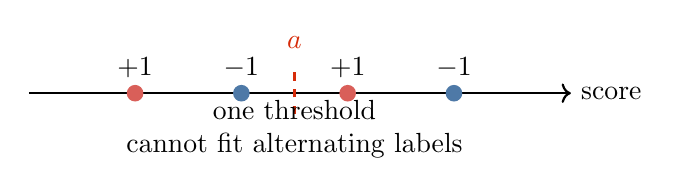
\begin{tikzpicture}[x=1.35cm,y=0.55cm]
        \draw[->,thick] (0,0) -- (5.1,0) node[right] {score};
        \foreach \x/\lab/\col in {1/+1/pointred,2/-1/pointblue,3/+1/pointred,4/-1/pointblue}{
          \fill[\col] (\x,0) circle (3pt);
          \node[above=2pt] at (\x,0) {$\lab$};
        }
        \draw[slideorange,very thick,dashed] (2.5,-0.48)--(2.5,0.48);
        \node[slideorange,above=5pt] at (2.5,0.48) {$a$};
        \node[align=center] at (2.5,-0.82) {one threshold\\cannot fit alternating labels};
      \end{tikzpicture}
      \end{center}
    \end{column}
    \begin{column}{0.35\textwidth}
      \KeyBox{\centering
        \textbf{Lookup rule}\\
        stores one decision per email\\[0.08cm]
        fits all four labels
      }
    \end{column}
  \end{columns}
  \vspace{0.10cm}
  \centering
  \textbf{Question:} which model class can correlate with random labels after seeing them?
\end{frame}

% V02 -- before original PDF page 12
\begin{frame}[t]{Visual: Repeated and Distinct Patients}
  \vspace{0.04cm}\small
  The same risk model can have different flexibility on different samples.
  \begin{center}
  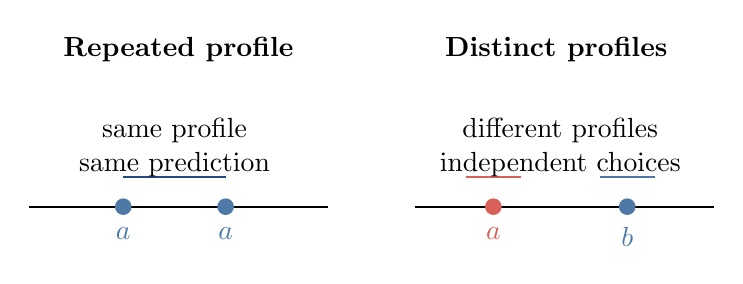
\begin{tikzpicture}[x=1cm,y=1cm]
    \node[font=\bfseries] at (1.9,2.0) {Repeated profile};
    \node[font=\bfseries] at (6.7,2.0) {Distinct profiles};
    \draw[thick] (0,0)--(3.8,0);
    \fill[pointblue] (1.2,0) circle (3pt) node[below=4pt] {$a$};
    \fill[pointblue] (2.5,0) circle (3pt) node[below=4pt] {$a$};
    \draw[deepblue,thick] (1.2,0.38)--(2.5,0.38);
    \node[align=center] at (1.85,0.75) {same profile\\same prediction};
    \draw[thick] (4.9,0)--(8.7,0);
    \fill[pointred] (5.9,0) circle (3pt) node[below=4pt] {$a$};
    \fill[pointblue] (7.6,0) circle (3pt) node[below=4pt] {$b$};
    \draw[pointred,thick] (5.55,0.38)--(6.25,0.38);
    \draw[pointblue,thick] (7.25,0.38)--(7.95,0.38);
    \node[align=center] at (6.75,0.75) {different profiles\\independent choices};
  \end{tikzpicture}
  \end{center}
  \vspace{0.08cm}
  \KeyBox{The first sample forces repeated evaluations to agree. The second
  sample lets the class choose two predictions separately.}
\end{frame}

% V03 -- before original PDF page 29
\begin{frame}[t]{Visual: Threshold and Interval Rules}
  \vspace{0.04cm}\small
  Two common rules over a one-dimensional measurement have different shapes.
  \begin{center}
  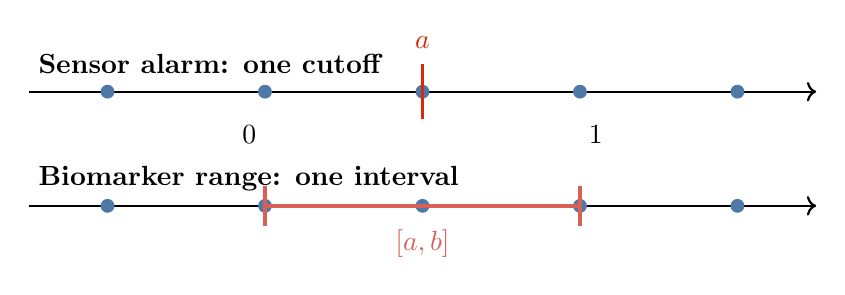
\begin{tikzpicture}[x=1.0cm,y=1cm]
    \node[anchor=west,font=\bfseries] at (0,1.35) {Sensor alarm: one cutoff};
    \draw[thick,->] (0,1)--(10,1);
    \foreach \x in {1,3,5,7,9}{\fill[pointblue] (\x,1) circle (2.5pt);}
    \draw[slideorange,very thick] (5,0.65)--(5,1.35);
    \node[slideorange,above=2pt] at (5,1.35) {$a$};
    \node at (2.8,0.45) {0};\node at (7.2,0.45) {1};
    \node[anchor=west,font=\bfseries] at (0,-0.10) {Biomarker range: one interval};
    \draw[thick,->] (0,-0.45)--(10,-0.45);
    \foreach \x in {1,3,5,7,9}{\fill[pointblue] (\x,-0.45) circle (2.5pt);}
    \draw[pointred,very thick] (3,-0.45)--(7,-0.45);
    \draw[pointred,very thick] (3,-0.70)--(3,-0.20);
    \draw[pointred,very thick] (7,-0.70)--(7,-0.20);
    \node[pointred,below=5pt] at (5,-0.45) {$[a,b]$};
  \end{tikzpicture}
  \end{center}
  \vspace{0.04cm}
  \centering
  Infinitely many parameter values can produce only finitely many behaviors on the observed points.
\end{frame}

% V04 -- before original PDF page 39
\begin{frame}[t]{Visual: Shattering as a Labeling Game}
  \vspace{0.04cm}\small
  Place the points first. Then ask whether the class can answer every labeling challenge.
  \begin{columns}[T,totalwidth=\textwidth]
    \begin{column}{0.52\textwidth}
      \textbf{Two points: all four challenges}
      \begin{center}
      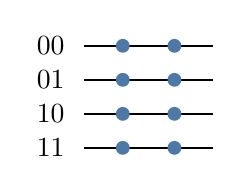
\begin{tikzpicture}[x=0.82cm,y=0.48cm]
        \foreach \y/\l in {3.0/00,2.1/01,1.2/10,0.3/11}{
          \node[anchor=east] at (-0.15,\y) {$\l$};
          \draw[thick] (0,\y)--(2,\y);
          \fill[pointblue] (0.6,\y) circle (2.5pt);
          \fill[pointblue] (1.4,\y) circle (2.5pt);
        }
      \end{tikzpicture}
      \end{center}
      Every labeling can be realized by a suitable interval.
    \end{column}
    \begin{column}{0.44\textwidth}
      \textbf{Three points: one challenge fails}
      \begin{center}
      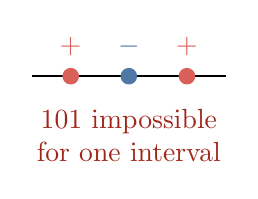
\begin{tikzpicture}[x=0.82cm]
        \draw[thick] (0,0)--(3,0);
        \fill[pointred] (0.6,0) circle (3pt) node[above=4pt] {$+$};
        \fill[pointblue] (1.5,0) circle (3pt) node[above=4pt] {$-$};
        \fill[pointred] (2.4,0) circle (3pt) node[above=4pt] {$+$};
        \node[darkred,align=center] at (1.5,-0.75) {$101$ impossible\\for one interval};
      \end{tikzpicture}
      \end{center}
    \end{column}
  \end{columns}
  \KeyBox{The largest number of points on which every labeling is possible is the VC dimension.}
\end{frame}

% V05 -- before original PDF page 44
\begin{frame}[t]{Visual: Linear Loan Boundary}
  \vspace{0.04cm}\small
  Let the axes represent income and debt. A linear approval rule is one side of a line.
  \begin{columns}[T,totalwidth=\textwidth]
    \begin{column}{0.55\textwidth}
      \begin{center}
      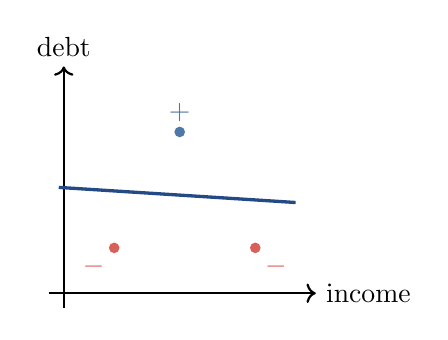
\begin{tikzpicture}[scale=0.64]
        \draw[->,thick] (-0.3,0)--(5.0,0) node[right] {income};
        \draw[->,thick] (0,-0.3)--(0,4.5) node[above] {debt};
        \fill[pointred] (1.0,0.9) circle (3pt) node[below left] {$-$};
        \fill[pointred] (3.8,0.9) circle (3pt) node[below right] {$-$};
        \fill[pointblue] (2.3,3.2) circle (3pt) node[above] {$+$};
        \draw[deepblue,very thick] (-0.1,2.1)--(4.6,1.8);
      \end{tikzpicture}
      \end{center}
    \end{column}
    \begin{column}{0.40\textwidth}
      \KeyBox{Three non-collinear customer profiles can realize every binary
      approval pattern by moving the line. Four profiles create a geometric
      obstruction, such as XOR.}
    \end{column}
  \end{columns}
  \vspace{0.04cm}
  \centering
  This is the geometric intuition behind VC dimension $3$ for affine separators in $\mathbb R^2$.
\end{frame}
\end{document}
